\documentclass{beamer}
%\usetheme{PaloAlto}
%\usetheme{Berlin}
\usetheme{Ilmenau}
\usecolortheme{seahorse}

%\usepackage[utf8]{inputenc}
%\usepackage{default}
%\usepackage[italian]{babel}

%\usepackage{titleref}
%\usepackage{zref-titleref}

\usepackage{amsmath}
\usepackage{amssymb}
\usepackage{amsthm}
\usepackage{xfrac}
\usepackage[all]{xy}
\usepackage{mathtools}
\usepackage{graphicx}
%\usepackage{fullpage}
\usepackage{hyperref}
\usepackage[utf8x]{inputenc}
\usepackage[italian]{babel}


%\usepackage{pdftricks}
%\begin{psinputs}
%   \usepackage[pdf]{pstricks}
 %  \usepackage{multido}
%\end{psinputs}

\usepackage{ulem}

\setlength{\parindent}{0in}

\newcounter{counter1}

\theoremstyle{plain}
\newtheorem{myteo}[counter1]{Teorema}
\newtheorem{mylem}[counter1]{Lemma}
\newtheorem{mypro}[counter1]{Proposizione}
\newtheorem{mycor}[counter1]{Corollario}
\newtheorem*{myteo*}{Teorema}
\newtheorem*{mylem*}{Lemma}
\newtheorem*{mypro*}{Proposizione}
\newtheorem*{mycor*}{Corollario}

\theoremstyle{definition}
\newtheorem{mydef}[counter1]{Definizione}
\newtheorem{myes}[counter1]{Esempio}
\newtheorem{myex}[counter1]{Esercizio}
\newtheorem*{mydef*}{Definizione}
\newtheorem*{myes*}{Esempio}
\newtheorem*{myex*}{Esercizio}

\theoremstyle{remark}
\newtheorem{mynot}[counter1]{Nota}
\newtheorem{myoss}[counter1]{Osservazione}
\newtheorem*{mynot*}{Nota}
\newtheorem*{myoss*}{Osservazione}

\newcommand{\obar}[1]{\overline{#1}}
\newcommand{\ubar}[1]{\underline{#1}}

\newcommand{\set}[1]{\left\{#1\right\}}
\newcommand{\pa}[1]{\left(#1\right)}
\newcommand{\ang}[1]{\left<#1\right>}
\newcommand{\bra}[1]{\left[#1\right]}
\newcommand{\abs}[1]{\left|#1\right|}
\newcommand{\norm}[1]{\left\|#1\right\|}

\newcommand{\pfrac}[2]{\pa{\frac{#1}{#2}}}
\newcommand{\bfrac}[2]{\bra{\frac{#1}{#2}}}
\newcommand{\psfrac}[2]{\pa{\sfrac{#1}{#2}}}
\newcommand{\bsfrac}[2]{\bra{\sfrac{#1}{#2}}}

\newcommand{\der}[2]{\frac{\partial #1}{\partial #2}}
\newcommand{\pder}[2]{\pfrac{\partial #1}{\partial #2}}
\newcommand{\sder}[2]{\sfrac{\partial #1}{\partial #2}}
\newcommand{\psder}[2]{\psfrac{\partial #1}{\partial #2}}

\newcommand{\intl}{\int \limits}

\DeclareMathOperator{\de}{d}
\DeclareMathOperator{\id}{Id}
\DeclareMathOperator{\len}{len}

\DeclareMathOperator{\gl}{GL}
\DeclareMathOperator{\aff}{Aff}
\DeclareMathOperator{\isom}{Isom}




\begin{document}


\title[Distanza di Hausdorff e applicazioni in computer
vision]{Distanza di Hausdorff e alcune applicazioni in computer
  vision}
%\subtitle{Proprietà degli spazi di forme}
%\author{Enrico Polesel}
\institute[Scuola Normale Superiore]{Scuola Normale Superiore}
\date{14 maggio 2014}

\author[Enrico Polesel]{\begin{tabular}{r@{ }l}
Autore: &  Enrico Polesel \\ 
Relatore: & Andrea Mennucci
\end{tabular}
}



\begin{frame}[plain]
  \titlepage
\end{frame}

\begin{frame}[plain]
 \frametitle{Indice}
 \tableofcontents
\end{frame}


%\AtBeginSection[]
%{
%  \begin{frame}{\secname}
%    \tableofcontents[currentsection]
%  \end{frame}
%}


\AtBeginSubsection[]
{
  \begin{frame}[plain]{\secname $\rightarrow$ \subsecname}
    \tableofcontents[currentsubsection]
  \end{frame}
}

\section{Spazi di forme}

\subsection{Distanza di un punto-insieme e rappresentazione delle forme}


\begin{frame}{Distanza da un insieme}
  Consideriamo $(M,d)$ spazio metrico e $\Omega \subseteq M$ spazio
  ``ambiente'' nel quale vogliamo considerare i sottoinsiemi.
  
  \begin{mydef}[Distanza di un punto da un insieme]
    Dato $A \subseteq \Omega$ non vuoto definiamo:
    
    \[  d_A (x) := \inf _{y \in A} d(x,y) \] 
  \end{mydef}
  
  Con questo possiamo rappresentare lo spazio di forme
  
  \[ C_d(\Omega) = \set{d_A : A \subseteq \Omega,\; A \neq \emptyset} \]
\end{frame}

\begin{frame}{Quando $d_A$ \`e in realt\`a un minimo}
  In generale l'$\inf$ della definizione della distanza $d_A$ non \`e
  un minimo, nemmeno chiedendo che $A$ sia chiuso, per esempio:
  \begin{myes}
    In $L^2(\mathbb{N})$ consideriamo i punti $a_n = ( 0, 0, ..., 1 +
    \frac{1}{n} , 0, ...)$ dove il termine non nullo si trova
    all'$n$-esimo posto. Allora $A = \set{ a_n : n\in \mathbb{N}}$ \`e
    chiuso, ma non esiste $a_n$ tale che $d(0,a_n)$ sia minimo
  \end{myes}

  L'$\inf$ diventa un minimo se:
  \begin{itemize}
  \item $A$ \`e compatto
  \item In $M$ le palle chiuse sono compatte e $A$ è chiuso
  \end{itemize}
\end{frame}

\begin{frame}{Proprietà della distanza da un insieme}
  \begin{mypro}[Proprietà della distanza punto-insieme]
    \begin{itemize}
    \item La funzione $x \rightarrow d_A(x)$ è 1-Lipschitz (e quindi
      continua)
    \item $d_{A\cup B}(x) = \min\set{d_A(x),d_B(x)}$
    \item $\set{x:d_A(x) = 0} = \obar A$
    \item $d_A \equiv 0 \Rightarrow A$ è denso in $\Omega$
    \item $d_{\obar A} = d_A$
    \item $A\subseteq B \Rightarrow d_A \ge d_B$
    \item $\obar{ A} \subseteq \obar B \Leftrightarrow d_A \ge d_B$
    \item $d_A = d_B \Leftrightarrow \obar A = \obar B$
    \end{itemize}
  \end{mypro}
\end{frame}

\begin{frame}{Spazio di forme}
  Classificare le forme $A \subseteq \Omega$ equivale a considerare i
  sottoinsiemi non vuoti di $\Omega$ a meno della chiusura, quindi
  possiamo prendere come rappresentanti delle forme le loro chiusure,
  cioè considerare l'insieme
  \[ C_s(\Omega) := \set{ A \subseteq \Omega : A = \obar A \wedge A
    \neq \emptyset } \]

  \begin{myoss}
    \[ C_s(\Omega) \cong C_d(\Omega) = \set{d_A : A \subseteq \Omega,\;
      A \neq \emptyset} \]
  \end{myoss}
  \vfill
  In certi casi saremo interessati a considerare solo i sottoinsiemi
  compatti di $\Omega$ che denotiamo con:
  \[ K(\Omega) = \set{K\subseteq \Omega :\; K \text{ compatto} \wedge
    A \neq \emptyset} \]
\end{frame}

\subsection{Distanza di Hausdorff}

\begin{frame}{Definizione}
  \begin{mydef}[Distanza di Hausdorff]
    Dati due insiemi $A,C \subseteq \Omega$ non vuoti definiamo
    \[ d_H(A,C) = \max \set{\sup _{x\in A} d_C (x) , \sup _{x\in C}
      d_A (x) } \]
\end{mydef}

In seguito dimostreremo che $d_H$ è effettivamente una distanza
\end{frame}

\begin{frame}{Definizioni equivalenti}
  Per semplicità di linguaggio definiamo%, usando una notazione analoga
  %a quella usata negli spazi vettoriali reali:
  \[ A + \obar B_\varepsilon := \set{ x \in \Omega : \exists y \in A :
    d(x,y) \le \varepsilon } \]
  Quando $A$ è chiuso si può scrivere anche
  \[ A + \obar B _{\varepsilon} = \set{ x \in \Omega \mid d_A(x) \le
    \varepsilon} \] 
  \begin{mypro}
    Dati $A, C \subseteq \Omega$ non vuoti le seguenti definizioni
    sono equivalenti
    \begin{enumerate}
    \item $ d_H (A,C) = \norm{ d_A - d_C } _\infty = \sup _{x\in \Omega}
      \set {d_A(x) - d_C(x)}$
    \item $d_H(A,C) = \max \set{\sup _{x\in A} d_C (x) , \sup _{x\in C}
        d_A (x) }$
    \item $d_H (A,C) = \inf \set{\delta : A \subseteq C + \obar B
        _\delta \wedge C \subseteq A + \obar B_\delta} = \max
      \set{\inf \set{\delta : A \subseteq C + \obar B _\delta }, \inf
        \set{\delta : C \subseteq A + \obar B _\delta }} $
    \end{enumerate}
  \end{mypro}
\end{frame}

\begin{frame}{La distanza di Hausdorff è una distanza}
%  Osserviamo che la distanza di Hausdorff non distingue fra un insieme
%  e la sua chiusura.
  \begin{mypro}
    Nell'insieme $C_s(\Omega)$ la funzione $d_H$ è una distanza
  \end{mypro}
  % \begin{proof}
  %   È ovvio che $d_H \ge 0$ e che $d_H(A,C) = d_H(C,A)$.

  %   \[d_H(A,C) = 0 \Leftrightarrow  \norm{d_A - d_C}_\infty = 0
  %   \Leftrightarrow d_A = d_C \Leftrightarrow \obar A = \obar C \]
    
  %   \[ \abs{d_A(x) - d_C(x)} \le \abs{d_A(x) - d_B(x)} + \abs{d_B(x) -
  %     d_C(x)} \le \] \[ \le d_H(A,B) + d_H(B,C) \]
  %   Da cui la tesi passando all'estremo superiore per $x\in \Omega$.
  % \end{proof}
%\end{frame}

%\begin{frame}{Ancora su $C_s(\Omega) \cong C _d (\Omega)$}
  \vfill
  Abbiamo dimostrato che $d_H$ è una distanza su $C_s(\Omega)$ perché
  la distanza di Hausdorff non distingue fra un insieme e la sua
  chiusura.
  \vfill
  Si ha inoltre:
  \begin{myoss}
    La relazione $C_s(\Omega) \cong C_d(\Omega)$ è un'isometria usando
    su $C_s(\Omega)$ la distanza di Hausdorff e la norma infinito su
    $C_d(\Omega)$
  \end{myoss}
\end{frame}

\subsection{Proprietà}

\begin{frame}{Completezza e compattezza}
  \begin{myteo}[Completezza]%{\cite[Proposizione 4.4.2]{ambrosio2000selected}}]
    Se $(\Omega,d)$ è completo allora $\pa{C_s(\Omega),d_H}$ è completo.
  \end{myteo}
  \vfill
%\end{frame}

%\begin{frame}{Compattezza}
  \begin{myteo}[Blaschke]%{\cite[Teorema 4.4.6]{ambrosio2000selected}}]
    % \label{teo:spazioformecompatto}
    Se $(\Omega,d)$ è compatto allora $\pa{C_s(\Omega),d_H}$ è compatto.
  \end{myteo}
  % \begin{proof}
  %   Per il teorema precedente $C_s(\Omega)$ è completo, quindi ci basta
  %   dimostrare che è anche totalmente limitato.
    
  %   Per farlo basta prendere $F = \set{f_1,...,f_n} \subseteq \Omega$ centri
  %   di una $\varepsilon$-rete finita che ricopre $\Omega$ e considerare
  %   $\mathcal{P}(F)$, questo insieme è ancora finito e si può dimostrare
  %   che è una $\varepsilon$-rete che ricopre $C_s(\Omega)$.
  % \end{proof}
\end{frame}

\begin{frame}{Numero di componenti connesse degli insiemi in
    $C_s(\Omega)$}
  \begin{mypro}
    La funzione $f:\; K(\Omega) \rightarrow \mathbb{N} \cup \set{+\infty}$
    che ad un compatto associa il numero delle sue componenti connesse è
    semicontinua inferiormente
  \end{mypro}
  \begin{mycor}
    Limite di compatti connessi è connesso.
  \end{mycor}
\end{frame}

\section{Geodetiche e metriche indotte}

\subsection{Distanza geodetica indotta}

\begin{frame}{Lunghezza di una curva}
  Sia $(M,d)$ uno spazio metrico
  \begin{mydef}
    Data $\gamma : \; \bra{a,b} \to M$ continua definiamo
    \[ \len^d \gamma := \sup _{\mathcal{P}_{fin}(\bra{a,b}) \ni T =
      \set{t_1 \le t_2 \le ... \le t_n}} \sum_{i=1}^n d\pa{
      \gamma\pa{t_{i-1}}, \gamma\pa{t_i}} \]
  \end{mydef}
  È facile vedere che, per la triangolare, si ha
  \[ \len^d \gamma \ge d\pa{\gamma\pa{a}, \gamma\pa{b}} \]

\end{frame}

\begin{frame}{Distanza geodetica indotta}
  Per semplicità di notazione definiamo
  \[ \Gamma (x,y) = \set{\gamma:\; \bra{a,b} \to M \mid
    \gamma(a) = x, \gamma(b) = y,\; \gamma \text{ continua}} \]
  
  \begin{mydef}[Distanza geodetica indotta]
    \[ d^g (x,y) := \inf _{\gamma \in \Gamma(x,y)} \len^d \gamma \]
  \end{mydef}

  Si vede facilmente che $d^g \ge d$, di conseguenza la topologia
  generata da $d^g$ è più fine di quella generata da $d$.
\end{frame}

\begin{frame}{Differenza tra $d$ e $d^g$}
  In generale non vale $d=d^g$ e la topologia indotta può essere molto
  diversa, per esempio

  \begin{figure}[h]
    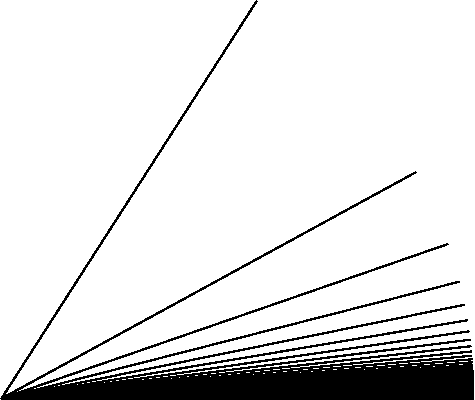
\includegraphics[scale=.7]{noncompattogeodetiche.pdf}
  \end{figure}
  % \begin{myes}%[{\cite[Esempio 2.1]{DuciMennucci2007}}]
  %   Sia $E = \bra{0,1} \times \pa{ \set{0} \cup \set{ \frac{1}{n} \mid n
  %       > 0} }$ e $\psi(\rho,\theta) = \rho
  %   \pa{\cos(\theta),\sin(\theta)}$. Considero quindi $M = \psi(E)$.
    
  %   $M$ è unione di segmenti di lunghezza $1$, passanti per l'origine
  %   con inclinazione decrescente che tendono al segmento orrizzontale
  %   (accumolandosi). 
    
  %   $M$ è compatto nella metrica euclidea, nella metrica indotta dalle
  %   geodetiche, però, $M$ non è più compatto, infatti i punti $x_n =
  %   \psi(1,\frac{1}{n})$ non posso ammettere una sottosuccessione
  %   convergente essendo, per ogni $n\neq m$, $d^g(x_n,y_m) = 2$.
  % \end{myes}
\end{frame}

% \begin{frame}
%   \begin{figure}[h]
%     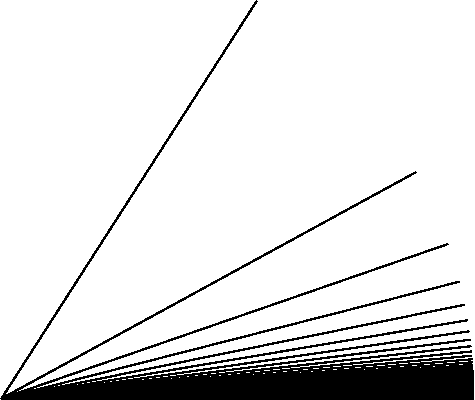
\includegraphics[scale=1]{noncompattogeodetiche.pdf}
%   \end{figure}
% \end{frame}

\begin{frame}{Metriche intrinseche}
  \begin{mydef}[Metrica intrinseca]
    Se la distanza $d$ è tale che $d = d^g$ si dice che $(M,d)$ è una
    metrica intrinseca
  \end{mydef}

  Per esempio $d^g$ è intrinseca
  \begin{mypro}
    \[\pa{d^g}^g = d^g\]
  \end{mypro}
\end{frame}

\subsection{Geodetiche}

% \begin{frame}{Lemmi}
%   \begin{mylem}
%     Data $\gamma:\; \bra{a,b} \to M$ continua si ha $\forall c \in
%     \pa{a,b}$ $\len ^d (\gamma_{|\bra{a,c}}) +  \len ^d (\gamma_{|\bra{c,b}}) = 
%     \len ^d (\gamma)$
%   \end{mylem}
%   \begin{mylem}
%     Se $\tilde \gamma \in \Gamma (x,y)$ con $\len ^d (\tilde \gamma) = L
%     < \infty$ e $\tilde \gamma : \; \bra {a,b} \to M$ allora si può
%     riparametrizzare $\tilde \gamma$ in $\gamma : \bra{0,L} \to M$ con la
%     proprietà $\len ^d(\gamma_{| \bra{0,t}}) = t$.
%   \end{mylem}
%   \begin{mylem}
%     Con la riparametrizzazione del lemma precedente si ha, presi $0 \le
%     t < s \le \len ^d (\gamma)$, che $\len ^d (\gamma _{|\bra{t,s}}) = s - t$
%   \end{mylem}
% \end{frame}

\begin{frame}{Geodetiche}
  \begin{mydef}[Geodetica]
    Dati $x,y \in M$ una curva $\gamma \in \Gamma\pa{x,y}$ è una
    geodetica se $\len ^d \gamma = d^g(x,y)$.
  \end{mydef}

  In generale non esistono sempre le geodetiche
  \begin{mylem}
    Se $M$ \`e compatto nella topologia indotta dalla metrica $d^g$
    allora $\forall x,y \in M$ esiste la geodetica che tra $x$ e $y$
    nella metrica indotta da $d$.
  \end{mylem}
\end{frame}

% \begin{frame}{Unicità della geodetica}
%   In generale le geodetica tra due punti non è unica
%   \begin{figure}[h]
%     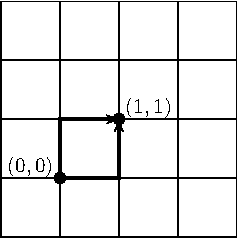
\includegraphics[scale=0.4]{griglia.pdf}
%   \end{figure}
%   In altri casi si ha anche l'unicità.
%   \begin{myes}
%     Sia $V$ uno spazio di Banach strettamente convesso, allora presi
%     comunque $x,y \in V$ l'unica geodetica è il segmento che li unisce.
%   \end{myes}
% \end{frame}

\subsection{Spazi di forme}

\begin{frame}{Metrica indotta}
  \begin{mypro}
    La metrica di $(M,d)$ è intrinseca se e solo se è intrinseca la
    metrica di $(C_s(M),d_H)$
  \end{mypro}
  % \begin{proof}
  %   Sia $d_H$ intrinseca, $x,y\in M$ e $\mu = d(x,y)$ e $\varepsilon
  %   >0$ possiamo definire induttivamente sull'insieme $Q = \set{ \mu
  %     \frac{k}{2^n}|\; 0< k <2^n\; k\text{ dispari}} \cup \set{0,\mu}$
  %   una funzione $\tilde \gamma$ tale che $d(\tilde \gamma(t), \tilde
  %   \gamma(s)) < \abs{s -t} + \varepsilon \frac{ \abs{ s-t}} {\mu}$ e
  %   poi estenerla per continuità ad una curva $\gamma \in \Gamma(x,y)$
  %   tale che $\len ^d (\gamma) < \mu + \varepsilon$.
  % \end{proof}
\end{frame}



% \begin{frame}
%   \begin{proof}
%     Se la metrica $d$ è intrinseca e $d_H(A,C) = \mu$ scelto
%     $\varepsilon >0$ ci basta considerare delle curve $\gamma _{(x,y)}
%     \in \Gamma (x,y)$ di lunghezza minore di $\mu + 2\varepsilon$ al
%     variare di $(x,y) \in \set{ (x,y) \in A\times C:\; d(x,y) < \mu +
%       \varepsilon }$ riparametrizzate da $\bra{0, \mu + 2\varepsilon}$
%     e definire una curva in $C_s(\Omega)$ come
%     \[ \obar G(t) = \obar {\set{ \gamma_{(x,y)}(t) : (x,y) \in P }} \]
%     Questa avrà lunghezza minore di $\mu + 2\varepsilon$.
%   \end{proof}
% \end{frame}

\begin{frame}{Esistenza}
  % \begin{mylem}
  %   Dati $x,y \in M$ esiste una geodetica tra di loro in $M$ se e solo
  %   se esiste in $B(x,d^g(x,y) + \delta)$ con $\delta > 0$
  %   qualsiasi.
  % \end{mylem}
  \begin{mypro}
    Se in $M$ le palle chiuse sono compatte nella metrica indotta
    allora esiste sempre la geodetica in $K(M)$ fra $A,C \in K(M)$.
  \end{mypro}
  % \begin{proof}
  %   Usando il lemma precedente mi restringo a cercare la geodetica in
  %   una palla chiusa sufficientemente grande, ma questa è compatta e
  %   quindi la geodetica esiste.
  % \end{proof}
\end{frame}
\begin{frame}{Unicità}
  In generale nella distanza di Hausdorff non si ha l'unicità della
  geodetica, ma in generale ne possono esistere più che numerabili
  \begin{figure}[h]
    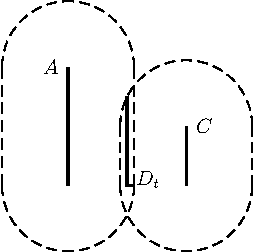
\includegraphics[scale=1]{geodetichehausdorff.pdf}
  \end{figure}
\end{frame}

\section{Distanza su spazi metrici quoziente}

\subsection{Proprietà}

\begin{frame}{Definizione}
  Sia $(M,d)$ uno spazio metrico e $G$ un gruppo che agisce su $M$
  \begin{mydef}[Distanza su $\sfrac{M}{G}$]
    \[ \obar d (\bra{x}, \bra{y}) = \inf _{\tilde x \in \bra{x} ,
      \tilde y \in \bra {y}} d(\tilde x , \tilde y) = \inf _ {g,h \in
      G} d(g(x), h(y)) \]
  \end{mydef}

  Questa funzione non è necessariamente una distanza, l'unica
  proprietà che verifica necessariamente è la simmetria
\end{frame}

% \begin{frame}{Chiusura delle orbite}
%   \begin{myoss}
%     Condizione necessaria perché $\obar d$ sia una distanza è che le
%     orbite di $G$ in $M$ siano chiuse
%   \end{myoss}
  
%   % Questa condizione non basta ancora per chiedere $\obar d(\bra{x},
%   % \bra{y}) = 0 \Leftrightarrow \bra{x} = \bra{y}$, una condizione
%   % sufficiente (ma non necessaria) è che le orbite siano
%   % compatte. Questa condizione non basta, però, per avere la
%   % disuguaglianza triangolare.
% \end{frame}

\begin{frame}{Invarianza di $d$ rispetto a $G$}
  \begin{mydef}
    Si dice che $d$ è invariante rispetto all'azione di $G$ se
    \[ \forall g \in G,\; \forall x,y \in M \;\; d(g(x),g(y)) = d(x,y) \]
  \end{mydef}
  Se $d$ è invariante rispetto a $G$ possiamo scrivere:
  \[ \obar d (\bra{x}, \bra{y}) = \inf _ {g,h \in G} d(g(x), h(y)) =
  \inf _{g \in G} d(x,g(y)) \]

  \begin{mypro}
    Se $d$ è invariante rispetto a $G$ allora $\obar d$ rispetta la
    disuguaglianza triangolare
  \end{mypro}
\end{frame}

\begin{frame}{Condizioni sufficienti per ottenere una distanza}
  \begin{mypro}
    Se $d$ è invariante rispetto a $G$ e le orbite sono chiuse allora
    $\obar d$ è una distanza
  \end{mypro}
  % \begin{proof}
  %   L'unica proprietà da dimostrare è $\obar d(\bra{x},
  %   \bra{y}) = 0 \Leftrightarrow \bra{x} = \bra{y}$, ma questa si
  %   verifica facilmente osservando che la relazione
  %   \[ 0 = \obar d(\bra{x},\bra{y}) = \inf _{g \in G} d(x,g(y)) \] 
  %   mostra che $x$ è aderente a $\bra{y}$.
  % \end{proof}
  Se non si chiede che le orbite siano chiuse vale comunque la
  triangolare e la simmetria, si ottiene quindi una pseudometrica.
\end{frame}

\begin{frame}{Topologia quoziente}
  \begin{mypro}
    Se $d$ è invariante per l'azione di $G$ e le orbite sono chiuse
    allora la topologia quoziente di $\sfrac{M}{G}$ coincide con la
    topologia data da $\obar d$.
  \end{mypro}

\end{frame}

% \begin{frame}{Passaggio di curve al quoziente}
%   \begin{mylem}
%     Ad ogni curva $\gamma \in \Gamma ( \bra{x}, \bra{y} )$ in $M$
%     possiamo associare una curva $\bra{\gamma} \in \Gamma( \bra{x},
%     \bra{y})$ tramite la proiezione al quoziente
%     \[ 
%     \xymatrix{I \ar[r]^\gamma \ar[dr] _{\obar \gamma}& M \ar[d]^\pi \\
%       & \sfrac{M}{G}  
%     }
%     \]
%     Inoltre $\len ^{\obar d} \pa{ \obar \gamma} \le \len ^d \pa{\gamma}$
%   \end{mylem}
% \end{frame}

\begin{frame}{Metrica geodetica indotta di $\obar d$}
  \begin{mypro}
    Se la metrica $d$ è intrinseca allora anche $\bar d$ è intrinseca.
  \end{mypro}
  \begin{mypro}
    Se le orbite sono compatte e $(M,d)$ è intrinseco allora
    l'esistenza delle geodetiche in $M$ implica l'esistenza delle
    geodetiche in $\sfrac{M}{G}$
  \end{mypro}
\end{frame}

\subsection{Il caso delle forme di $\mathbb{R}^N$}

\begin{frame}{Azione di un'affinità}
  Considero $\mathbb{R}^N$ con la distanza euclidea.
  \begin{mydef}
    Dato $A \in C_s(\mathbb{R}^N)$ e $g \in \aff (\mathbb{R}^N)$
    definisco
    \[ g(A) = \set{ g(a) \mid a \in A } \]
  \end{mydef}
  Ha senso chiedersi sotto quali ipotesi questa funzione sia continua
  nello spazio delle forme
\end{frame}

\begin{frame}{Continuità dell'azione}
  \begin{mypro}
    Se $A \in C_s(\mathbb{R}^N)$ allora la funzione $f: \mathbb{R}^N \to
    C_s(\mathbb{R}^N)$ tale che $f(t) = A + t := \set { a + t \mid a \in
      A}$ è continua.
  \end{mypro}
  \begin{mypro}
    Se $A \in K(\mathbb{R}^N)$ allora $\forall G < \gl (\mathbb{R}^N)$
    l'azione $f: G \rightarrow K(\mathbb{R}^N)$ tale che $f(g) = g(A)$
    è continua
  \end{mypro}
  \begin{mycor}
    Scelto $A \in K(\mathbb{R}^N)$ la funzione $f:\; \aff( \mathbb{R}^N)
    \to K(\mathbb{R}^N)$ tale che $f(g) = g(A)$ è continua.
  \end{mycor}
\end{frame}

\begin{frame}{Invarianza della distanza di Hausdorff con l'azione
    delle isometrie}
  \begin{myoss}
    La distanza di Hausdorff su $K(\mathbb{R}^N)$ è invariante per
    l'azione del gruppo delle isometrie di $\mathbb{R}^N$
  \end{myoss}

  Quindi, per dimostrare che $\obar d$ è una distanza su
  $\sfrac{K(\mathbb{R}^N)}{G}$ mi basta ora dimostrare che le orbite
  sono chiuse
\end{frame}

\begin{frame}{Preliminari}
  \begin{mylem}
    Sia $A \in K(\mathbb{R}^N)$ e $\pa{ g_n} _{n \in \mathbb{N}}
    \subseteq \isom( \mathbb{R}^N)$ tale che $\pa{ g_n(A) } _{n \in
      \mathbb{N}}$ è una successione convergente, allora esiste $\delta
    < \infty$ tale che, le isometrie $\pa{ g_n} _{n\in \mathbb{N}}$
    utilizzano traslazioni di norma minore di $\delta$.
  \end{mylem}
  \begin{mylem}
    Il gruppo ortogonale 
    \[ O(\mathbb{R},N) = \set{ M \in \gl (\mathbb{R},N) \mid M M^t =
      \id } \]
    è compatto $\forall N \in \mathbb{N}$.
  \end{mylem}
\end{frame}

\begin{frame}{Chiusura delle orbite}
  \begin{mypro}
    Dato $G \subseteq \isom(\mathbb{R}^N)$ chiuso le orbite generate
    dalla sua azione su $K(\mathbb{R}^N)$ sono chiuse.
  \end{mypro}
  % \begin{proof}
  %   Prendendo un punto di accumulazione si vede che i punti possono
  %   essere visti come immagini di un sottogruppo compatto di $\isom
  %   (\mathbb{R}^N)$ e quindi il limite appartiene all'orbita
  % \end{proof}
  \begin{mycor}
    Su $\sfrac{K(\mathbb{R}^N)}{G}$ la funzione $\obar d$ è
    effettivamente una distanza
  \end{mycor}
\end{frame}

\begin{frame}{Altre proprietà}
  \begin{myoss}
    Si vede facilmente che, dati $A,C \in K(\mathbb{R}^N)$, esiste $g
    \in G$ tale che $d_H \pa{A, g(C)} = \bar d _H \pa{ \bra{A},
      \bra{C}}$.
  \end{myoss}
  Inoltre, applicando i risultati precedenti
  \begin{mycor}
    In $\sfrac{K(\mathbb{R}^N)}{G}$ 
    \[ \obar{d} ^g = \obar{d} \]
  \end{mycor}
\end{frame}

\section{Ricerca di un ``punto medio''}


\subsection{Media basata sulle distanze}

\begin{frame}{Definizione}
  Sia, al solito, $(M,d)$ uno spazio metrico
  \begin{mydef}
    Dati $a_1,a_2,... a_n \in M$ diciamo che $\obar a$ è \textbf{un}
    punto medio se è un minimo per la funzione
    \[ m_A (a) = \sum _{i = 1} ^n d(a,a_i)^2 \]
  \end{mydef}
  
  Ha senso discutere l'esistenza e l'unicità di tale punto caso per
  caso, infatti potrebbe non esistere e, quando esiste, potrebbe non
  essere unico.

  \begin{myoss}
    La funzione $m_A$ è continua.
  \end{myoss}
\end{frame}

%\subsection{Spazi di forme}

\begin{frame}{Spazi di forme}
  \begin{mypro}
    Dati $A_1, A_2,..., A_n \in K(\mathbb{R}^N)$ esiste $A \in
    K(\mathbb{R}^N)$ che minimizza la funzione
    \[ m(A) = \sum _{i =1} ^n d(A,A_i)^2 \]
  \end{mypro}

  \begin{mypro}
    Dato $G < \isom (\mathbb{R}^N)$ e $A_1,...,A_n \in K(\mathbb{R}^N)$
    esiste $A \in K(\mathbb{R}^N)$ che minimizza la funzione 
    \[ \obar m(\bra{A}) = \sum _{i =1} ^n \obar
    d_H(\bra{A},\bra{A_i})^2 \]
  \end{mypro}
\end{frame}


\section{Applicazioni}

\subsection{Riconoscimento di forme}

\begin{frame}{Il problema}
  Siano $\mathcal{A} = \set{ A_1,...,A_n} \subseteq K(\mathbb{R^N})$
  forme di uno stesso tipo, data $A \in K(\mathbb{R}^N)$ ci chiediamo
  quanto sia simile alle forme in $\mathcal{A}$.
\end{frame}

\begin{frame}{La soluzione}
  Definiamo quindi una forma ``media'' (chiamiamola $\obar A$) come
  una delle medie basate sulla distanza di $\mathcal{A}$ e una
  varianza empirica come:

  \[ S^2 = \frac{1}{N-1} \sum _{i=1} ^n d_H(A_i , \obar A)^2 =
  \frac{1}{N-1} m(\obar A) \]

  Avendo quindi una media $\obar A$ e una varianza (empirica) $S$
  possiamo costruire un test statistico per dire quanto $A$ è simile
  alle forme di $\mathcal{A}$ in cui confrontiamo $d_H(\obar A, A)$
  con $S$.
\end{frame}


\subsection{Classificazione di forme}

\begin{frame}{Diagramma di Voronoi}
  \begin{mydef}[Diagramma di Voronoi]
    Dato $(M,d)$ spazio metrico e $x_1,...,x_k \in M$ punti distinti
    definiamo diagramma di Voronoi il partizionamento
    \[ R_j = \set{ x\in M : \forall 1 \le i \le k \;\; d(x,x_j) \le
      d(x,x_i) } \]
  \end{mydef}
\end{frame}

\begin{frame}{Il problema}
  Supponiamo di avere $k$ tipi di forme (compatte) e $n$ campioni
  $\mathcal{A} = \set{ A_1, A_2,..., A_n} \in K(\mathbb{R}^N)$ di esse,
  vorremmo dividerli in $k$ insiemi $S_1,...,S_k$, uno per tipo. Che
  proprietà deve avere tale partizione?
\end{frame}

\begin{frame}{Un criterio di ottimalità}
  Per ogni insieme $S_j$ di punti vogliamo intanto scegliere un
  rappresentate, per farlo scegliamo un punto medio basato sulla
  distanza, sia esso $M_j$. Ha senso ora calcolare
  \[ m_j = \sum _{A\in S_j} d(M_j,S_j)^2 \]
  
  \vfill

  Ci aspettiamo che un criterio di ottimalità sia la quantità
  \[ \sum _{j=1} ^k m_j \]
\end{frame}

\begin{frame}{Definizione del clustering}
  Se $M_1,...,M_k$ sono dei candidati rappresentanti, partizioniamo lo
  spazio nel diagramma di Voronoi $R_1,...,R_k$ e quindi i campioni in
  \[ S_j = \mathcal{A} \cap R_j \]
  
  \vfill

  A questo punto definiamo la funzione obbiettivo come
  \[ f(M_1,...,M_k) = \sum _{j = 1} ^k m_j = \sum _{j = 1} ^k \pa{ \sum
    _{A \in S_j} d(A,M_j)^2 } \]
\end{frame}

\begin{frame}{Clustering}
  Poniamoci come obbiettivo, quindi, trovare $M_1,...,M_k \in
  K(\mathbb{R}^N)$ che siano un minimo di $f$.
  
  \vfill

  Tale approccio ha due difetti:
  \begin{itemize}
  \item il numero di forme $k$ è un dato in ingresso
  \item il problema così posto è NP-hard
  \end{itemize}
\end{frame}





\end{document}







